\section{Background}
\label{sec:background}
This Section provides an overview of the research that 
underlies the main results of the thesis. Specifically, in this Section we will explore
the concepts of dataflow analysis, control-flow analysis, attribute grammars, 
and their implementation through the JastAdd framework.

Dataflow analysis is a technique used to determine the values that are used and 
defined within a program. It is a fundamental concept in the field of compiler 
construction, and it is used to optimize code and to security threats and bugs. 
Dataflow analysis depends on control-flow analysis, which computes an overapproxiamation of
all possible paths that a program can take.

Attribute grammars are a formalism for describing the structure of a program, 
and for specifying properties of the program. They are used in the implementation 
of compilers, and program analysis tools.
Reference Attribute Grammars (RAGs) is a particular kind of attribute grammars 
where the attribute values are defined in terms of references to the attributes 
of other elements in the grammar. JastAdd which is used in our work is a meta-compiler 
for implementing compilers and other language tools, e.g., static analysers, using RAGs.

The main results of this thesis are IntraCFG and JFeature. 
IntraCFG is a language-independent framework for implementing control-flow graphs 
on the source code level.
It is based on JastAdd and Control-flow analysis theory. IntraTeal is a instance
of IntraCFG on the TEAL language that we will use to demonstrate the effectiveness
of the framework. We also designed JFeature, a fact extractor for Java programs,
with the aim of presenting a more comprehensive overview of a Java program by 
taking into account the utilisation of various features and constructs specific 
to the Java language across different Java versions. The objective of JFeature is
to assist researchers and developers in the process of selecting benchmarks.

Throughout this Section, these concepts will be discussed in more detail and used to 
demonstrate the effectiveness of the proposed methods.

% Here we can use different styles to distinguish between the different types of nodes
% Everything is already set up, we just need to use the right style
\begin{figure}[h]
    \centering
    \scalebox{0.8}{
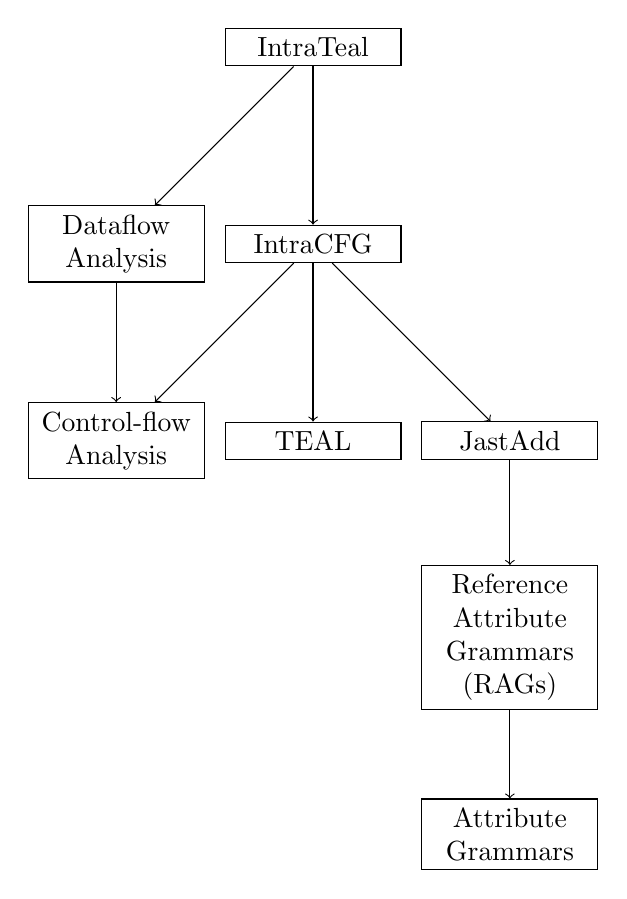
\begin{tikzpicture}[ 
    node distance=2.5cm,
    results/.style={rectangle,draw=black,text width=2cm,text centered},
    rags/.style={rectangle,draw=black,text width=2cm,text centered},
    analysis/.style={rectangle,draw=black,text width=2cm,text centered},
    teal/.style={rectangle,draw=black,text width=2cm,text centered}]
    \node[analysis] (dataflow) {Dataflow Analysis};
    \node[analysis, below of = dataflow] (cfa) {Control-flow Analysis};
    \node[results, right of = dataflow] (intracfg) {IntraCFG};
    \node[teal, below of = intracfg] (teal) {TEAL};
	\node[rags, right of = teal] (jastadd) {JastAdd};
    \node[rags, below of = jastadd] (rags) {Reference Attribute Grammars (RAGs)};
	\node[rags, below of = rags] (ags) {Attribute Grammars};
    \node[results, above of = intracfg] (intrateal) {IntraTeal};
    \path[->] (dataflow) edge (cfa);
    \path[->] (jastadd) edge (rags);
    \path[->] (rags) edge (ags);
    \path[->] (intracfg) edge (cfa);
    \path[->] (intracfg) edge (teal);
    \path[->] (intracfg) edge (jastadd);
    \path[->] (intrateal) edge (dataflow);
    \path[->] (intrateal) edge (intracfg);
  \end{tikzpicture}}
  \caption{Dependency graph of the concepts discussed in this Section.}
\end{figure}


\subsection{Control-flow analysis}

Control-flow analysis involves analysing the control flow of the program, which refers
to the execution order of the program's statements. It aids in comprehending the logical
structure of a program and recognising potential flaws, such as uninitialized variables
and infinite loops. Control-flow analysis
can provide valuable insights into the structure and behaviour of a program,
which can help with program understanding and maintenance.
% However, it is not always possible to establish the exact control flow of a program
% due to the Rice-Turing theorem, which is a key limitation of control-flow analysis.
We can distinguish two main approaches to constructing the control-flow graph (CFG) for a program:
on the source-level and on the intermediate representation. The source-level approach
involves analysing the source code of a program and constructing the control-flow graph
directly from the source code on top of the abstract syntax tree. The intermediate representation approach involves
first converting the source code into an intermediate representation, e.g., bytecode,
and then constructing the control-flow graph from the intermediate representation.

Constructing the control-flow graph on the source level has several advantages.
One of the main benefits is that it allows for the analysis to be performed directly
on the source code of the program, which can be more easily understood by humans.
This can be particularly useful for debugging and program understanding tasks,
as it allows the analysis to be performed in the context of the original program.
Another advantage of constructing the CFG on the source level is that it does not
require the generation of an intermediate representation (IR). This can make the
analysis faster and more efficient, as it avoids the overhead of IR generation.
In addition, constructing the CFG on the source level can work with semantically
and syntactically broken code, which can be useful for analysing programs with
errors or inconsistencies.
Furthermore, in situations where the IR must be generated in real-time,
for instance, when the analysis is performed in an integrated development environment (IDE),
the overhead of code generation and optimization may make this process too expensive,
causing latency in the IDE and frustration in the developer.
In such cases, constructing the control-flow graph (CFG) on the source level
may be a more efficient option.

However, there are also some disadvantages to constructing the CFG on the source level.
One of the main limitations is that it can be more difficult to accurately capture the
control-flow of a program when working with the source code it may contain constructs,
such as macros and preprocessor directives, that
can complicate the analysis. In addition, the source code may be written in a variety
of languages with different syntax and semantics, which can make it challenging to
design a single analysis that works across all languages.
The examples in Figures~\ref{fig:cfgsourcelevel} and~\ref{fig:cfgintermediatelevel} show the control-flow
graphs of the simple \texttt{foo} method.
\begin{figure}[h]
  \centering
\begin{tabular}{l r}
  \begin{lstlisting}[language=JastAdd]
void foo(){
  int x = 0;
  if (x > 0) {
    x = 1;
  } else {
    x = -1;
  }
}
  \end{lstlisting} &\hspace{2.5cm}
  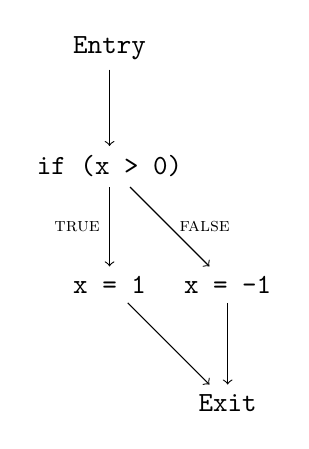
\begin{tikzpicture}[node distance=1.5cm, baseline=(current bounding box.center)]
      \node (start) [rectangle] {\texttt{Entry}};
      \node (if) [rectangle, below of=start] {\texttt{if (x > 0)}};
      \node (then) [rectangle, below of=if] {\texttt{x = 1}};
      \node (else) [rectangle, right of=then] {\texttt{x = -1}};
      \node (end) [rectangle, below of=else] {\texttt{Exit}};
      \draw [->] (start) -- (if);
      \draw [->] (if) -- node [left, font=\scriptsize] {\textsc{true}} (then);
      \draw [->] (if) -- node [right,  font=\scriptsize]{\textsc{false}} (else);
      \draw [->] (then) -- (end);
      \draw [->] (else) -- (end);
  \end{tikzpicture}
  \end{tabular}
  \caption{\label{fig:cfgsourcelevel}Source level control-flow graph of the \texttt{foo} method, showing the branching behavior of the if statement.}
\end{figure}


\begin{figure}[h]
  \centering
\begin{tabular}{l r}

\begin{lstlisting}[language=bytecode, frame=none]
0 : iconst_0
1 : istore_1
2 : iload_1
3 : ifle        10
6 : iconst_1
7 : istore_1
8 : goto        13
11: iconst_m1
12: istore_1
13: return
\end{lstlisting}
&\hspace{2.5cm}
\begin{tikzpicture}[
  node distance=0.4cm,
  every node/.style={shape=rectangle, align=center},
  baseline=(current bounding box.center)]
  % Nodes
  \node (0) {0};
  \node (1) [below=of 0] {1};
  \node (2) [below=of 1] {2};
  \node (3) [below=of 2] {3};
  \node (6) [left=of 3] {6};
  \node (7) [below=of 6] {7};
  \node (8) [below=of 7] {8};
  \node (11) [right=of 3] {11};
  \node (12) [below=of 11] {12};
  \node (14) [below=of 3] {};
  \node (15) [below=of 14] {};
  \node (13) [below=of 15] {13};

  % Edges
  \path[->] (0) edge (1) (1) edge (2) (2) edge (3) (3) edge[bend right] (6) (3) edge[bend left] (11) (6) edge (7) (7) edge (8) (8) edge (13) (11) edge (12) (12) edge (13);

  \draw[dashed] (0.north west) rectangle (2.south east);
  \draw[dashed] (6.north west) rectangle (8.south east);
  \draw[dashed] (11.north west) rectangle (12.south east);

\end{tikzpicture}
\end{tabular}
\caption{\label{fig:cfgintermediatelevel}Bytecode control-flow graph of the \texttt{foo} method. Each dashed box represents a basic block.}
\end{figure}




\subsection{Dataflow Analysis}
\label{sec:dataflowanalysis}
Dataflow analysis is a technique used in computer science to analyse the flow of
data through a program. It has its roots in the field of program optimization,
where it was originally used to identify opportunities for improving the performance
of programs by removing unnecessary computations e.g., Very Busy Expression or Available Expression analyses~\cite{aho2007compilers,vallee-rai10soot,falconer2007deepweaver,sagiv1996ide,kildall1973dataflow}.
Dataflow analysis involves tracking the flow of data through a program by
identifying the variables that are defined and used at each point in the program's
control flow. This information can be used to optimize the program by eliminating
unnecessary computations and improving the use of available resources.
One of the primary advantages of dataflow analysis is its ability to handle programs
with complex control flow, such as those with loops and conditional statements.

In the context of bug detection~\cite{spoon, fink2012wala}, dataflow analysis can be used to identify
potential sources of errors in a program by tracking the flow of data through
the program and identifying points where data may be used in unexpected or
incorrect ways. This can be particularly useful in identifying bugs that may
not be immediately apparent, such as those that only occur under certain
conditions or when certain combinations of input data are used.
Many tools for static analysis of Java programs, such as FindBugs~\cite{findbugs},
SpotBugs~\cite{spotbugs}, and PMD~\cite{copeland2005pmd}, use dataflow analysis to identify
potential bugs in Java programs.
% I looked here how they cited pmd, findbugs and spotbugs. https://ieeexplore.ieee.org/stamp/stamp.jsp?tp=&arnumber=8103456

Dataflow analysis can also be used to identify potential security vulnerabilities
in software~\cite{flowDroid,piskachev2021secucheck,lawall10coccinelle}. By tracking the flow of sensitive data through a program and
identifying points where it may be exposed to unauthorized access or manipulation,
dataflow analysis can help to identify potential vulnerabilities that could be
exploited by attackers.

\subsubsection*{Monotone Frameworks}
Monotone framework~\cite{kam1977monotone} is a teoretical framework for reasoning about program dataflow properties.
These frameworks provide a flexible and generic framework for expressing and solving
dataflow equations, which can be used to reason about a wide range of dataflow 
properties, such as live variables, reaching definitions, and available expressions analyses.
Monotone frameworks are built on the concept of lattice~\cite{Donnellan1968,Birkhoff1967,cousot1977ai}. 
A lattice is a partially ordered set in which any two elements have a unique least 
upper bound (also known as a join or a supremum) and a unique greatest lower bound 
(also known as a meet or an infimum). Meaning that, any elements a and b in 
the lattice, there exists a unique element denoted as a $\vee$ b (or a $\cup$ b) 
such that a $\leq$ a $\vee$ b and b $\leq$ a $\vee$ b, and a $\wedge$ b 
(or a $\cap$ b) such that a $\wedge$ b $\leq$ a and a $\wedge$ b $\leq$ b.

A well-formed lattice has a unique least element, commonly denoted as $\bot$, 
and a unique greatest element, commonly denoted as $\top$. These elements satisfy 
the properties that for any element $x$ in the lattice, $\bot \leq x$ and x $\leq \top$.
The diagram in Figure~\ref{fig:lattice} shows the lattice of sets over the set
$S = \{s_1, s_2, s_3\}$, where the partial ordering is defined by set inclusion
and the least upper bound and greatest lower bound are set union and set intersection
respectively. The least element in this lattice is the empty set $\emptyset$ and the
greatest element is the set $S$ itself. 

A forward monotone framework consist of two equations and a transfer function $f$.
For each node $n$ in the control-flow graph, we define the following two equations:
$$\text{in}(n) = \bigcup\limits_{p \in \text{pred}(n)} \text{out}(p)$$

$$\text{out}(n) = f(\text{in}(n), n)$$

where $f:C \mapsto L$ is a monotone transfer function, also called transfer function. 
The transfer function $f$ maps each element $c$ in the set $C$ (i.e., concrete domain) 
to an element $f(c)$ in the lattice $L$ (i.e., abstract domain). $pred(n)$ and $succ(n)$ 
denote the set of predecessors and successors of node $n$, respectively.

A backward monotone framework is similar to a forward framework, except that the equations are reversed:
$$\text{out}(n) = \bigcup\limits_{s \in \text{succ}(n)} \text{in}(s)$$

$$\text{in}(n) = f(\text{out}(n), n).$$

The framework defines a mutual dependency between the $in$ and $out$ sets of a node.
This circular dependency is solved through a fix point computation.
Fix point computation is a mathematical technique that finds a stable 
state, or fix point, in a system. In the context of the Monotone framework, this 
refers to finding a state where the $in$ and $out$ sets of all nodes in the CFG have reached a 
stable value, and no further changes will occur. The fix point is guarantee to exist
because the transfer function $f$ is monotone~\cite{Knaster1929}.




\begin{figure}[h]
    \centering
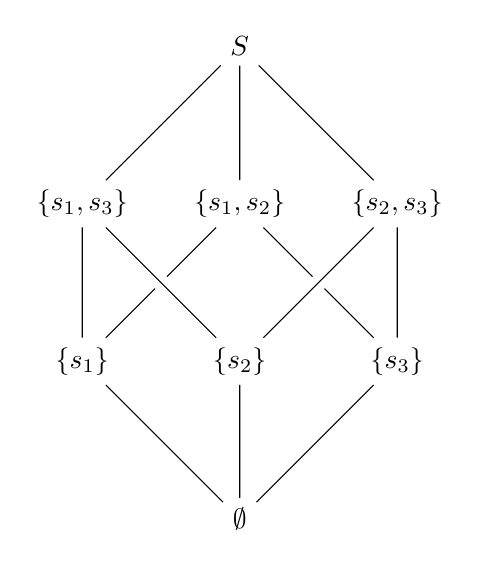
\begin{tikzpicture}
    \node (max) at (0,4) {$S$};
    \node (a) at (-2,2) {$\{s_1,s_3\}$};
    \node (b) at (0,2) {$\{s_1,s_2\}$};
    \node (c) at (2,2) {$\{s_2,s_3\}$};
    \node (d) at (-2,0) {$\{s_1\}$};
    \node (e) at (0,0) {$\{s_2\}$};
    \node (f) at (2,0) {$\{s_3\}$};
    \node (min) at (0,-2) {$\emptyset$};
    \draw (min) -- (d) -- (a) -- (max) -- (b) -- (f)
    (e) -- (min) -- (f) -- (c) -- (max)
    (d) -- (b);
    \draw[preaction={draw=white, -,line width=6pt}] (a) -- (e) -- (c);
  \end{tikzpicture}
  \caption{\label{fig:lattice}Hesse diagram~\cite{Hesse1874} of the $\mathcal{P}(S)$ lattice.
  In this case, $S = \top$ and $\emptyset = \bot$.}
\end{figure}

\subsection{Attribute Grammars}
\label{chap:attr-grammars}
Attribute grammars~\cite{knuth1968semantics} (AGs) are a formalism for specifying
the syntax and semantics of programming languages.
They were first introduced by Knuth in 1968 as a way to define the syntax and semantics of the programming
language ALGOL 68. This formalism is based on the concept of attributes,
which are properties associated with the elements of a language's abstract syntax tree.
Attribute grammars provide a powerful tool for specifying the behaviour of a programming
language and for verifying the correctness of programs written in that language.
%
ARs are composed of two components: a context-free grammar~\cite{CREMERS197586},
which defines the syntax of the language, and an attribute evaluation function,
which defines the semantics of the language. The context-free grammar is used to
parse a program into its abstract syntax tree, and the attribute evaluation function
is used to compute the values of the attributes associated with each element
of the tree.

A key advantage of attribute grammars is their ability to capture the
interdependence of syntactic and semantic elements of a programming language.
For example, the type of a variable may be determined by its declaration,
but the type of an expression may be determined by the types of its subexpressions.
Attribute grammars provide a way to specify these constraints.

Attributes are define using equations. We can distinguish two types of
attributes: synthesized attributes and inherited attributes.
For the sake of readability, we borrow the notation introduced by Fors et al. in~\cite{fors2020patterns},
where attribute names are preceded by a symbol that indicates the type of the attribute.
We reserve the symbol \Abase{x} to denote the attribute name and the symbol $e$ to denote the attribute value,
e.g., a constant, a function of the node's children, or a function of the node's children
and the node's own attributes.

A \emph{synthesized} attribute is a property of a non-terminal that is computed
based on the attributes of its possible derivations. For example, the type of an expression
in a programming language may be a synthesized attribute that is computed based
on the types of the subexpressions in the expression. For instance, if a variable is initialized
with the expression ``3 + 4'', the type of the variable would be determined to
be integer based on the types of the operands in the expression.

\begin{equation*}
  \Asyn{A}{x} = e
  \end{equation*}
where \astnode{A} is the name of the node type.

An \emph{inherited} attribute is a property of a non-terminal that is inherited from
its parent element in the abstract syntax tree. For example, the scope of a variable
in a programming language may be an inherited attribute that is inherited from the
scope in which the variable is declared.
An example of an inherited attribute is the scope of a variable in a programming
language. The scope of a variable is the region of a program in which the variable
is visible and can be accessed. The scope of a variable is inherited from the
context in which it is declared. For example, if a variable is declared within a
function, the variable will be visible and accessible within the body of the function,
but not outside of the function.


Inherited attributes are defined by two parts: a declaration and an equation.
\begin{equation*}
\Ainh{A}{x} \quad\quad \quad\quad \Ainhdef{B}{*}{x} = e
\end{equation*}
where \astnode{A} and \astnode{B} are node types.
The first part of the equation declares the attribute \Ainh{A}{x} as inherited by \astnode{A},
so that every node of type \astnode{A} has can access it. The second part of the
equation defines the attribute for each child of \astnode{B}. The whildcard \astnode{*}
indicates that the attribute is defined and broadcasted to all children of \astnode{B} with type \astnode{A}.

\begin{figure}
    \begin{tikzpicture}[scale=0.7,edge from parent/.style={draw,-latex},sibling distance=8em,
      every node/.style = {align=center,scale=1},
      astnode/.style={shape=rectangle, draw, fill=white, minimum width=5mm,%
      minimum height=10mm},
      synthesized/.style={shape=rectangle, draw, fill=orange!15},
      inherited/.style={shape=rectangle, draw, fill=blue!15}
      ]

    \node [astnode,draw] (A) {\code{A}}
      child {node [astnode] (B) {\code{B}}}
      child {node [astnode] (C) {\code{C}}
    }
    ;
    \node [synthesized , draw, right=0pt of A] (AA) {\Asyn{A}{z} = \Asyn{B}{x} + 1 = 3};
    \node [synthesized , draw, left=0pt of B] (BB) {\Asyn{B}{x} = 2};
    \node [synthesized , draw, right=0pt of C] (CC) {\Asyn{C}{v} = 5};
    \node [inherited , draw, below right =0pt of C] (CC) {\Ainh{C}{y} = \Asyn{A}{z} + \Asyn{C}{v} = 8};

    \matrix [draw, below right = -50pt and -180pt,inner sep=1ex,cells={nodes={font=\sffamily,anchor=west}}] at (B) {
      \node [synthesized] {}; & \node{Synthesized attributes}; \\
      \node [inherited] {}; & \node{Inherited attributes}; \\
      \node [rectangle,draw] {}; & \node{AST Node}; \\
      \draw[-latex,dotted,color=black](0,0) -- ++ (0.3,0); & \node{Child relation}; \\
    };
    \end{tikzpicture}
    \caption{\label{fig:ragsExample} Graphical representation of the attribute grammar example.}
\end{figure}

Let us consider the following abstract grammar:

    \begin{align*}
        A& ::= B \quad C \\
        B& \\
        C&
    \end{align*}

and the following attribute declarations:
    \begin{align*}
        \Asyn{A}{z}& = \Asyn{B}{x} + 1 \\
        \Asyn{B}{x}& = 2 \\
        \Asyn{C}{v}& = 5 \\
        \Ainh{C}{y}& \\
        \Ainhdef{A}{C}{y}& = \Asyn{A}{z} + \Asyn{C}{v} \\
    \end{align*}
The value for the synthesized attribute \Asyn{A}{z} is computed by solving
the equation systems for the attributes \Asyn{A}{z} and \Asyn{B}{x}:
\begin{align*}
    \Asyn{A}{z} &= \Asyn{B}{x} + 1 \\
    \Asyn{B}{x} &= 2
\end{align*}
leading to \Asyn{A}{z} = 3 and \Asyn{B}{x} = 2.
The value for the inherited attribute \Ainh{C}{y} is defined by the node \astnode{A} for
each child of type \astnode{C}. The value of \Ainh{C}{y} is computed by solving the equation system:
\begin{align*}
    \Ainh{C}{y} &= \Asyn{A}{z} + \Asyn{C}{v} \\
    \Asyn{C}{v} &= 5\\
    \Asyn{A}{z} &= 3
\end{align*}
resulting in \Ainh{C}{y} = 8. Figure~\ref{fig:ragsExample} depicts the described example.


\subsection{Reference Attribute Grammars}
\label{sec:rag}
Reference Attribute Grammars (RAGs) where introduced in~\cite{DBLP:journals/informaticaSI/Hedin00}
and are an extension of Attribute Grammars to Object-Oriented languages. While attributes in Attribute Grammars
can only refer to terminal values, RAGs allow attributes to refer to non-terminals i.e., node in the AST.
RAGs are well-suited for the analysis of object-oriented languages, since they enable
the definition of relation between AST nodes. Attributes that refer to
to AST nodes can declaratively construct relation, i.e., graphs, on the AST.
Examples of the relations that can be constructed using RAGs are:
\begin{itemize}
    \item Name analysis: checks that all names are well-defined and used correctly. A relation between
    the name and the definition of the name is constructed,
    \item Type analysis: checks that all expressions have a valid type. A relation between the expression
    and its type is constructed,
    \item Graph of a class hierarchy: a graph where nodes are classes and edges are inheritance relations,
    \item Control flow graph: a graph where nodes are statements and/or expressions, and edges are control flow relations, and,
    \item Call graph: a graph where nodes are methods and edges are method calls.
\end{itemize}

\subsection{The TEAL Programming Language}
TEAL (Typed Easily Analysable Language) is a programming language designed by Christoph Reichenbach, and  used in the
program analysis\footnote{\url{https://fileadmin.cs.lth.se/cs/Education/EDAP15/2022/web/index.html}} course at Lund University.
It is a simplified version of Java and its grammar and some aspects of its semantics are
listed in Appendix~TBD.  %Not sure if we should include the grammar in the thesis or just cite it.
One of the key features of TEAL is that it is an object-oriented language,
which means that it allows the creation of classes and objects that can inherit
characteristics and behavior from one another. However, it does not have a dynamic
dispatcher, which means that the method that is called for an object at runtime
is determined at compile time based on the type of the object.
In addition to supporting the definition of new types, TEAL also allows the use
of arrays. It was developed in an incremental manner, with each version building
upon the features of the previous one. TEAL-0 is the most basic version and includes
support for variable declarations and use, procedures, and basic control structures such as if
and while statements. TEAL-1 introduces the enhanced-for loop, and TEAL-2 allows users to
define their own types.

Overall, the goal of TEAL is to provide a language that allows students to
focus on the challenges of performing program analysis on a real-world language
without being overwhelmed by the details of a fully-featured language.
For the sake of simplicity, we will use TEAL-0 and TEAL-1 to exemplyfy the use of RAGs 
and the main results summarized in this thesis.

\subsection{The JastAdd Metacompiler}
\label{sec:jastadd}
The JastAdd metacompiler~\cite{DBLP:journals/entcs/HedinM01} is a tool for the construction of
Reference Attribute Grammars. The JastAdd metacompiler is a Java-based tool that generates
Java code from a RAG. The generated code can be used to construct an AST and to perform
analysis on the AST.
The JastAdd metacompiler is based on the following components:
\begin{itemize}
    \item The JastAdd language: a language for the definition of RAGs.
    The JastAdd language allow to specify the abstract grammar of a language, and,
    with a java-like syntax, the attributes of the RAG.
    \item The JastAdd compiler: a compiler that generates Java code from a RAG.
\end{itemize}
In JastAdd, synthesized attributs are defined using the \code{syn} keyword followed
by the type and the name of the attribute. Similarly, inherited attributes are defined
using the \code{inh} keyword. Let us reconsider the example depicted in Figure~\ref{fig:ragsExample}.
The abstract grammar is defined in a \code{.ast} file with the following syntax:
    \begin{lstlisting}[language=JastAdd]
        A ::= B C;
        B;
        C;
    \end{lstlisting}
where each line defines a non-terminal, i.e., a node in the AST.
The attributes are defined in a \code{.jrag} file with the following syntax:
    \begin{lstlisting}[language=JastAdd]
        syn int A.z() = B.x() + 1;
        syn int B.x() = 2;
        syn int C.v() = 5;
        inh int C.y();
        eq A.C.y() = A.z() + C.v();
    \end{lstlisting}
The last line is an equation that defines the value of the inherited attribute \Ainh{C}{y} for each child of type \astnode{C}.
\begin{figure}
    \begin{center}
        \begin{tikzpicture}
            \tikzstyle{block} = [rectangle, draw, text centered, minimum height=8em, minimum width=8em]
            \tikzstyle{line} = [draw, -latex]
            \node [block] (A) {
                \begin{lstlisting}[language=JastAdd]
aspect AttrDecl {
  syn int A.x() = 1;
  syn int B.x() = 2;
}
                \end{lstlisting}
            };
            \node [block, right=of A, yshift=5em] (B) {
                \begin{lstlisting}[language=JastAdd]
class A {
    public int x(){
    return 1;
    }
}
                \end{lstlisting}
            };
            \node [block, below=of B] (C) {
                \begin{lstlisting}[language=JastAdd]
class B {
    public int x(){
        return 2;
    }
}
                  \end{lstlisting}
             };

             \node (v1) at (-1.9,-0.05) {};
             \node (v2) at (2,-0.05) {};
             \node (v3) at (3.8,1.1) {};
             \node (v4) at (7.1,1.1) {};
             \node (v5) at (7.1,2.3) {};
             \node (v6) at (3.8,2.3) {};
             \node (v7) at (2,0.3) {};
             \node (v8) at (-1.9,0.3) {};
             \draw[opacity=0.2,fill=blue] (v1.center)--(v2.center)--(v3.center)--(v4.center)--(v5.center)--(v6.center)--(v7.center)--(v8.center)--(v1.center);

             \fill [opacity=0.2,blue]
                 (v1) \foreach \i in {2,...,8}{ -- (v\i) } -- cycle;

            \node (vv1) at (-1.9,-0.1) {};
            \node (vv2) at (2,-0.1) {};
            \node (vv3) at (3.8,-1.5) {};
            \node (vv4) at (7.1,-1.5) {};
            \node (vv5) at (7.1,-2.8) {};
            \node (vv6) at (3.8,-2.8) {};
            \node (vv7) at (2,-0.45) {};
            \node (vv8) at (-1.9,-0.45) {};
            \draw[opacity=0.2,fill=red] (vv1.center)--(vv2.center)--(vv3.center)--(vv4.center)--(vv5.center)--(vv6.center)--(vv7.center)--(vv8.center)--(vv1.center);

            \fill [opacity=0.2,red]
                (v1) \foreach \i in {2,...,8}{ -- (vv\i) } -- cycle;
        \end{tikzpicture}
    \end{center}
    \caption{\label{fig:interType} Example of intertype declaration.}
\end{figure}


JastAdd supports intertype declarations for the definition of attributes. An intertype declaration
of an attribute is a declaration that is performed into an aspect that, at compile time,
is inlined in the class specified in the intertype declaration. The example in Figure~\ref{fig:interType}
shows an intertype declaration of an attribute.
The attributes \Asyn{A}{x} and \Asyn{B}{x} are defined in the aspect \code{AttrDecl}
that is inlined in the classes \code{A} and \code{B} respectively.

JastAdd supports not only synthesized and inherited attributes, but also:
\begin{itemize}
    \item \emph{Parametrised Attribute}: the value of the attribute might depend
    not only on the AST node itself, but also on the value of the arguments supplied
    to it. Attributes of this kind are widely used, especially in the definition of
    type-checking rules.
    \begin{lstlisting}[language=JastAdd]
syn boolean Type.compatibleType(Type t){
    return this==t;
}
    \end{lstlisting}


    \item \emph{Higher-Order Attribute (HOA)}\footnote{Also known as \emph{Non-Terminal Attributes (NTA)}.}:
    the value of an HOA is a freshly new subtree. Are called \emph{Higher-Order Attributes}
    because are attribute and at the same time a non-terminal, therefore they can be attributed.
    The subtree computed by an HOA behaves like a normal non-terminal, i.e., it can be
    attributed and it can be used in the definition of other attributes. In JastAdd, HOAs
    are defined using the \code{nta} keyword. HOAs are widely used to reify information
    that are not explicit in the source-code and therefore, not present in the AST.
    For example, when constructing a CFG of a method, is always useful to specify
    a unique entry point and a unique exit point for the method. In JastAdd, this can be
    achived using an HOA:
    \begin{lstlisting}[language=JastAdd]
syn nta Entry MethodDecl.entry() = new Entry();
syn nta Exit MethodDecl.exit() = new Exit();
    \end{lstlisting}
    We use the right-arrow symbol to denote HOAs, e.g.,  \Ahoa{MethodDecl}{entry} and \Ahoa{MethodDecl}{exit}.
    \item \emph{Circular Attribute}: an attribute which definition might depend direclty
    or indirectly on itself. In JastaAdd, circular attributes are expressed using the \code{circular}
    keyword. To guarantee termination, circular attributes are evaluated in a fixed-point
    computation, i.e., the attribute is evaluated until the value of the attribute does not change.
    The requirements, that are not checked by JastAdd, to guarantee termination are:
    \begin{itemize}
        \item All the possible values computed by the attribute must be placed
        in a lattice of finite height.
        \item The intermediate results of the fix-point algorithm must increase
        or decrease monotonically\footnote{In this Thesis, boolean circular attributes start
        as \emph{false} and monotonically grow with $\vee$, while set-typed circular attributes
        start as the empty set and monotonically grow with $\cup$.}.
    \end{itemize}
    We use the symbol \AcircSyn{A}{x} to denote a circular synthesized attribute.

    \item \emph{Collection Attribute}: have no equations, but contributions. The
    result of a collection attribute is the aggreatation of contributions that can
    come frome anywhere else in the AST. A contribution clause is associated with
    an AST node type and describes information to be included in a collection
    attribute, possibly under certain conditions. Collection attributes, are expecially
    useful in compiler construction, to collect all the semantic errors in a program
    from anywhere in the AST. In JastAdd, collection attributes are defined using the
    \code{coll} keyword. For example, the following collection attribute collects all
    the type errors in a program:
    \begin{lstlisting}[language=JastAdd]
coll Set<Errors> Program.errors();
Expr contributes  when type.compatibleType(expectedType()) to Program.errors();
    \end{lstlisting}
    We use the following notation to denote the collection attribute \code{errors}: \Acoll{Program}{errors}.
\end{itemize}




